%!TEX root = ../prak.tex
\section{Lab 5 Dinierende Philosophen}
Das Problem der dinierenden Philosophen ist ein klassisches Synchronisationsproblem. In Abbildung 1 ist die Konfiguration mit drei Philosophen dargestellt. Das Problem lautet wie folgt: Einige Philosophen sitzen an einem runden Tisch und essen Nudeln. Zu ihrer Linken und Rechten befindet sich je ein Stäbchen, das sie mit ihrem Nachbarn teilen. Insgesamt befinden sich nur so viele Stäbchen wie Philosophen auf dem Tisch. Die Philosophen machen den ganzen Tag nichts anderes als zu denken, zu essen, wieder zu denken, etc. Wenn ein Philosoph essen will, muss er beide Stäbchen benutzen. Wenn einer seiner Nachbarn ein Stäbchen besitzt, muss er warten, bis beide Stäbchen frei sind. Obwohl alle Philosophen unterschiedlich schnell denken, kann der Fall eintreten, dass mehrere gleichzeitig essen wollen.

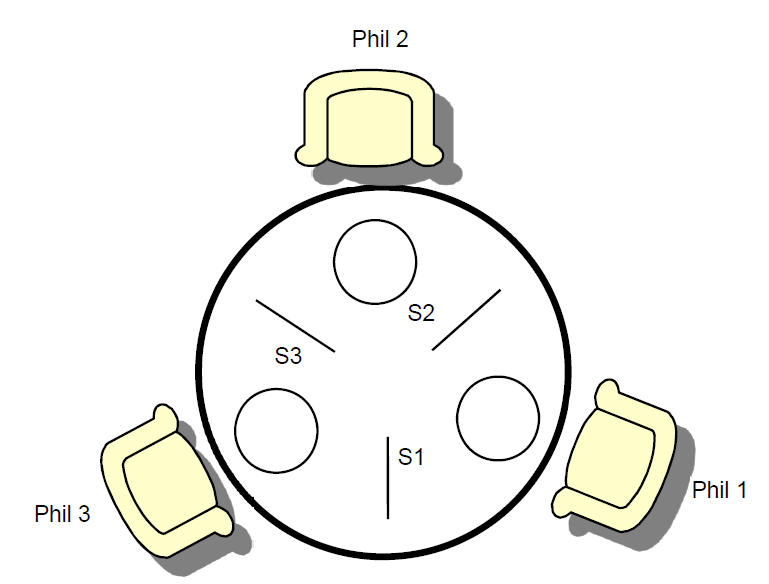
\includegraphics[width=.4\linewidth]{900-Praktika/prak05/pic.PNG}


\subsection{Aufgabe 1: Untersuchung von Deadlocks}
Untersuchen Sie die folgenden Fälle auf Verklemmungen (Deadlocks). Formulieren Sie eine verklemmungsfreie
Regel, bzw. welche der Varianten würden Sie implementieren? Die Regeln müssen so gestaltet werden,
dass die Philosophen während der "Synchronisation" ohne Absprachen untereinander auskommen, d.h.
bei Kenntnis dieser Regeln kann jeder Philosoph selbständig handeln.

\begin{enumerate}
  \item Jeder hungrige Philosoph nimmt seine beiden Stäbchen gleichzeitig auf, sobald beide verfügbar sind. Falls nur eines verfügbar ist, lässt er dieses auf dem Tisch liegen.
  \item Jeder hungrige Philosoph nimmt zuerst das Stäbchen links von seinem Teller auf. Das Stäbchen rechts von seinem Teller nimmt er nur dann auf, wenn er das linke schon hat.
  \item Alle Stäbchen werden durchnummeriert. Jeder hungrige Philosoph nimmt zuerst das Stäbchen mit der kleineren Nummer bei seinem Teller. Das Stäbchen mit der grösseren Nummer nimmt er nur dann auf, wenn er das Stäbchen mit der kleineren Nummer schon besitzt.
\end{enumerate}

\subsubsection{Lösung}

\begin{enumerate}
  \item Diese Variante funktioniert. Entweder nimmt der Philosoph gar kein Stäbchen oder zwei aufs Mal. Er muss einfach noch beide aufs Mal fassen können. Das könnte zu Problemen führen.
  \item Diese Variante funktioniert überhaupt nicht. Wenn alle Philosophen Hunger haben, nimmt jeder das linke Stäbchen und alle warten auf das zweite, welches aber keiner freigeben wird. Ein typischer Deadlock
  \item Diese Variante funktioniert, obwohl sie sehr ähnlich zu Variante b) aussieht. Die Regel gegen Deadlock lautet, dass alle die Ressourcen in der ganz genau gleichen Reihenfolge anfordern müssen. Zuerst links, dann rechts gemäss b) widerspricht dem. In b) will Phil 1 zuerst S1, dann S2, Phil 2 nimmt zuerst S2, dann S3, Phil 3 nimmt hingegen zuerst S3, dann S1. Hier liegt das Problem. In c) fordern Phil 1 und Phil 2 die Ressourcen genau gleich an wie in b). Phil 3 fordert aber zuerst S1 und dann S3 an, d.h. immer in derselben Reihenfolge.
\end{enumerate}

\subsection{Aufgabe 2: Implementation der dinierenden Philosophen}

m Verzeichnis ./Vorgabe/Philo finden Sie eine Codevorgabe für fünf Philosophen. Das main() ist sehr komfortabel: es müssen nur Objekte der Klasse Philosopher definiert werden. Diese Klasse bietet nur die beiden Elementfunktionen live() und join() an. Alles weitere, insbesondere die Erzeugung des Threadkontexts, ist intern in der Klasse umgesetzt. Studieren Sie den Code in Philosopher.h.

\begin{lstlisting}[language=C++, style=C++]
class Philosopher
{
  public:
    Philosopher(int pid, int thinkdelay, int eatDelay, Sticks& s);
    ~Philosopher();
    void live();       // the philosopher's life
    void join();       // wait for philosopher to leave
  private:
    enum {nMeals = 3};
    int id;            // this philosopher's id
    int tDelay;        // how long does this philosopher think?
    int eDelay;        // how long does this philosopher eat?
    int left;          // left fork number
    int right;         // right fork number
    Sticks& stick;     // sticks used by all philosophers
    pthread_attr_t attr;
    pthread_t tid;     // thread id
    void lifeThread(); // the (C++) - thread function
    static void* staticWrapper(void* p) // C Wrapper for pthread_create()
    {                                   // p must be the this pointer
        static_cast<Philosopher*>(p) -> lifeThread();
        return 0;
    }
};
\end{lstlisting}

\begin{enumerate}
  \item Erläutern Sie die Elementfunktion \texttt{Philosopher::lifeThread()}. Wozu dient sie?
  \item Erklären Sie die Funktion \texttt{Philosopher::staticWrapper()}. Wieso braucht es diese Funktion, was ist ihre Aufgabe und welche Beziehung hat diese Funktion zu \texttt{Philosopher::lifeThread()}?
  \item Schreiben Sie ein Programm in C++, welches das Philosophenleben simuliert und für alle fünf Philosophen gleich fair ist. Ein Deadlock darf nie eintreten. Implementieren Sie jeden Philosophen als Thread in\newline\texttt{Philosopher::live()}, die Denkphase können Sie mit einer jeweils zufällig gewählten Schlafdauer umsetzen. Den Zugriff auf die Stäbchen müssen Sie in der Klasse Sticks als Monitor implementieren, d.h. alle Locks müssen in dieser Klasse mit \texttt{pthread\_mutex\_lock()}, bzw. \texttt{pthread\_mutex\_unlock()} gemacht werden, der Aufrufer muss sich nicht darum kümmern müssen. Eine Condition Variable braucht es hier ebenfalls.
  \item In der Monitorklasse Sticks verwenden Sie bisher direkt die C-Funktionen \texttt{pthread\_mutex\_lock()}, bzw. \texttt{pthread\_mutex\_unlock()}. Setzen Sie jetzt RAII (Resource Acquisition Is Initialization) ein. Beachten Sie dazu auch die Klasse \texttt{ResourceLock} aus dem Praktikum 10 (Aufgabe 3) vom Modul Embedded Software Engineering 1.
\end{enumerate}

\subsubsection{Lösung}

\begin{enumerate}
  \item Die Elementfunktion \texttt{Philosopher::lifeThread()} ist die Threadfunktion, d.h. sie beinhaltet den Code, den ein Thread auszuführen hat. Sie hat den Zugriff auf sämtliche (auch privaten) Attribute und Funktionen der Klasse Philosopher. Sie zeigt, wie auch in C++ eine Elementfunktion als Threadfunktion genutzt werden kann.
  \item Ein Thread muss mit der C-Funktion \texttt{pthread\_create()} gestartet werden. Diese Funktion benötigt als Parameter einen Funktionspointer auf eine C-Funktion, welche die Threadfunktion beinhaltet. Die statische C++-Funktion \texttt{Philosopher::staticWrapper()} liegt ausserhalb des Klassenkontextes und kann der Funktion \texttt{pthread\_create()} übergeben werden. Der Static Wrapper ruft im Objektkontext die Elementfunktion \texttt{Philosopher::lifeThread()} auf. Den Objektkontext erhält der Wrapper über den void-Pointer. Deshalb muss der Funktion \texttt{pthread\_create()} der this-Pointer (das ist der Objektkontext) übergeben werden: \texttt{pthread\_create(\&tid, \&attr, staticWrapper, this);}
  \item siehe ./Loesung/Philo Bei der Ausführung bemerken Sie allenfalls, dass cout nicht thread-safe ist. Einzelne Texte mögen auseinandergerissen (interleaved) sein.

\lstinputlisting[language=C++, style=C++, multicols=2]{900-Praktika/prak05/Loesung/Philo/sticks.h}
\noindent\makebox[\linewidth]{\rule{\paperwidth}{0.4pt}}
\lstinputlisting[language=C++, style=C++, multicols=2]{900-Praktika/prak05/Loesung/Philo/sticks.cpp}
\noindent\makebox[\linewidth]{\rule{\paperwidth}{0.4pt}}
\lstinputlisting[language=C++, style=C++, multicols=2]{900-Praktika/prak05/Loesung/Philo/Philosopher.h}
\noindent\makebox[\linewidth]{\rule{\paperwidth}{0.4pt}}
\lstinputlisting[language=C++, style=C++, multicols=2]{900-Praktika/prak05/Loesung/Philo/Philosopher.cpp}
\noindent\makebox[\linewidth]{\rule{\paperwidth}{0.4pt}}
\lstinputlisting[language=C++, style=C++, multicols=2]{900-Praktika/prak05/Loesung/Philo/PhiloTest.cpp}

  \item siehe ./Loesung/PhiloRAII Sie benötigen die Klasse ResourceLock. Ein Objekt dieser Klasse müssen Sie in den beiden Elementfunktionen \texttt{Sticks::get()} und \texttt{Sticks::put()} einsetzen. Der Rest bleibt sich gleich.
\end{enumerate}

\lstinputlisting[language=C++, style=C++, multicols=2]{900-Praktika/prak05/Loesung/PhiloRAII/ResourceLock.h}
\noindent\makebox[\linewidth]{\rule{\paperwidth}{0.4pt}}
\lstinputlisting[language=C++, style=C++, multicols=2]{900-Praktika/prak05/Loesung/PhiloRAII/sticks.h}
\noindent\makebox[\linewidth]{\rule{\paperwidth}{0.4pt}}
\lstinputlisting[language=C++, style=C++, multicols=2]{900-Praktika/prak05/Loesung/PhiloRAII/sticks.cpp}
\noindent\makebox[\linewidth]{\rule{\paperwidth}{0.4pt}}
\lstinputlisting[language=C++, style=C++, multicols=2]{900-Praktika/prak05/Loesung/PhiloRAII/Philosopher.h}
\noindent\makebox[\linewidth]{\rule{\paperwidth}{0.4pt}}
\lstinputlisting[language=C++, style=C++, multicols=2]{900-Praktika/prak05/Loesung/PhiloRAII/Philosopher.cpp}
\noindent\makebox[\linewidth]{\rule{\paperwidth}{0.4pt}}
\lstinputlisting[language=C++, style=C++, multicols=2]{900-Praktika/prak05/Loesung/PhiloRAII/PhiloTest.cpp}
